%%%%%%%%%%%%%%%%%%%%%%%%%%%%%%%%%%%%%%%%%%%%%%%%%%%
%% P3: Phenomenology of Particle Physics                         
%%
%% Author:  André Rubbia                   		 
%%
%% Figure 26.13 Total cross-section for $e^+e^-\rightarrow W^+W^-$ in picobarns as a function of the center-of-mass energy.
%%
%% This work is licensed under the Creative Commons Attribution 4.0 International License. 
%% To view a copy of this license, visit http://creativecommons.org/licenses/by/4.0/ or 
%% send a letter to Creative Commons, PO Box 1866, Mountain View, CA 94042, USA.
%%
%%%%%%%%%%%%%%%%%%%%%%%%%%%%%%%%%%%%%%%%%%%%%%%%%%%

\documentclass[a4paper,10pt]{article}

\usepackage[T1]{fontenc}
\usepackage[utf8]{inputenc}
\usepackage{lmodern}
\usepackage[labelfont=bf]{caption}
\usepackage{upgreek}

\usepackage{tikz}
\usepackage{pgfplots}
\pgfplotsset{compat=1.17}
\usepgfplotslibrary{ternary}
\usepgfplotslibrary{fillbetween}
\usepgfplotslibrary{external}

\def\d{\mathrm{d}}
\setlength{\oddsidemargin}{-1.0cm}
\setlength{\evensidemargin}{-1.0cm}
\setlength{\textheight}{25cm}
\setlength{\textwidth}{18cm}

\begin{document}

%%%%%%%%%%%%%%%%   FIGURE  %%%%%%%%%%%%%%%%%%%%%%%%%%%%%%
\begin{figure}[htb]
\pgfplotsset{every axis/.append
    style={
%    font=\large,
    line width=1pt,
    tick style={line width=0.8pt}}}
\begin{tikzpicture}[scale=1.2]
    \begin{axis}[
        title=$e^+e^-\rightarrow W^+W^-$,
        xlabel={$\sqrt{s}$ (GeV)},
        ylabel={$\sigma$~(pb)},
        xmin=150, xmax=500,
        ymin = 0, ymax=40,
        minor y tick num=1,
        grid = major,
        legend entries={
        all diagrams,
        only $\nu_e$-exchange channel,
        no $ZWW$ diagram,
        },
        legend style={legend pos = outer north east}
    ]
\addplot[
    color=blue
    ]
    coordinates {
(162,5.62274)
(163,7.45795)
(164,8.81324)
(165,9.89552)
(166,10.7936)
(167,11.5561)
(168,12.2132)
(169,12.7853)
(170,13.2872)
(171,13.7299)
(172,14.1218)
(173,14.47)
(174,14.7798)
(175,15.0558)
(176,15.3019)
(177,15.5213)
(178,15.7167)
(179,15.8907)
(180,16.0452)
(181,16.1821)
(182,16.303)
(183,16.4094)
(184,16.5025)
(185,16.5835)
(186,16.6534)
(187,16.7131)
(188,16.7635)
(189,16.8052)
(190,16.8391)
(191,16.8656)
(192,16.8854)
(193,16.899)
(194,16.9069)
(195,16.9095)
(196,16.9071)
(197,16.9003)
(198,16.8892)
(199,16.8743)
(200,16.8558)
(201,16.834)
(202,16.809)
(203,16.7813)
(204,16.7508)
(205,16.718)
(206,16.6829)
(207,16.6457)
(208,16.6065)
(209,16.5656)
(210,16.523)
(211,16.4788)
(212,16.4333)
(213,16.3865)
(214,16.3385)
(215,16.2893)
(216,16.2392)
(217,16.1881)
(218,16.1362)
(219,16.0835)
(220,16.0301)
(221,15.9761)
(222,15.9215)
(223,15.8664)
(224,15.8107)
(225,15.7547)
(226,15.6983)
(227,15.6415)
(228,15.5845)
(229,15.5272)
(230,15.4696)
(231,15.4119)
(232,15.354)
(233,15.296)
(234,15.2379)
(235,15.1798)
(236,15.1215)
(237,15.0633)
(238,15.005)
(239,14.9467)
(240,14.8885)
(241,14.8304)
(242,14.7723)
(243,14.7142)
(244,14.6563)
(245,14.5985)
(246,14.5408)
(247,14.4832)
(248,14.4258)
(249,14.3685)
(250,14.3114)
(251,14.2544)
(252,14.1977)
(253,14.1411)
(254,14.0847)
(255,14.0285)
(256,13.9726)
(257,13.9168)
(258,13.8613)
(259,13.8059)
(260,13.7509)
(261,13.696)
(262,13.6414)
(263,13.587)
(264,13.5328)
(265,13.4789)
(266,13.4253)
(267,13.3719)
(268,13.3187)
(269,13.2658)
(270,13.2132)
(271,13.1608)
(272,13.1087)
(273,13.0568)
(274,13.0052)
(275,12.9539)
(276,12.9028)
(277,12.852)
(278,12.8014)
(279,12.7511)
(280,12.7011)
(281,12.6514)
(282,12.6019)
(283,12.5526)
(284,12.5036)
(285,12.4549)
(286,12.4065)
(287,12.3583)
(288,12.3104)
(289,12.2627)
(290,12.2153)
(291,12.1682)
(292,12.1213)
(293,12.0747)
(294,12.0283)
(295,11.9822)
(296,11.9364)
(297,11.8908)
(298,11.8454)
(299,11.8003)
(300,11.7555)
(301,11.7109)
(302,11.6665)
(303,11.6224)
(304,11.5786)
(305,11.535)
(306,11.4916)
(307,11.4485)
(308,11.4056)
(309,11.363)
(312,11.2365)
(322,10.83)
(332,10.4455)
(342,10.0817)
(352,9.73736)
(362,9.41104)
(372,9.10159)
(382,8.80787)
(392,8.52884)
(402,8.26353)
(412,8.01104)
(422,7.77056)
(432,7.5413)
(442,7.32257)
(452,7.11373)
(462,6.91416)
(472,6.72332)
(482,6.54069)
(492,6.36579)
    };

\addplot[
    color=red, dashed,
    ]
    coordinates {
(162,	5.80353)
(172,	18.4504)
(182,	25.9225)
(192,	31.7538)
(202,	36.5933)
(212,	40.7418)
(222,	44.3829)
(232,	47.6431)
};

\addplot[
    color=magenta, dotted,
    ]
    coordinates {
(162,	5.72073)
(172,	16.452)
(182,	21.4482)
(192,	24.7921)
(202,	27.2759)
(212,	29.2353)
(222,	30.8505)
(232,	32.2307)
(242,	33.4475)
(252,	34.5498)
(262,	35.5728)
(272,	36.5421)
(282,	37.4769)
(292,	38.3918)
(302,	39.2979)
(312,	40.2041)
};


  \end{axis}
\end{tikzpicture}%
\caption{Total cross-section for $e^+e^-\rightarrow W^+W^-$ in picobarns as a function
of the center-of-mass energy $\sqrt{s}$. The dashed curve shows the contribution
from the $\nu_e$-exchange $t$-channel. The dotted curve includes the
$\nu_e$ exchange and the $\gamma WW$ diagram. The continuous line includes all contributions.
}
	\end{figure}
%
%%%%%%%%%%%%%%%%   END FIGURE  %%%%%%%%%%%%%%%%%%%%%%%%%%%%%%
%
\end{document}
